\chapter{Background\label{Background}}

This chapter examines the challenges of diagnosing rare diseases, of
the databases we harvest data from and of the data models we intend to
use, including applied optimized heuristics. We will reason our
choices through the preliminary work of others and look at
alternatives to some of the choices made. We will also go through
selected parts of the theoretical aspects of the methods used in our prototype
system.

\section{Diagnosing rare diseases}

In theory, clinical decision-making is a complicated process based on
experience, judgement and a reasoning coming from a large integrate of
medical literature and clinical trials. In practise though, a
physician may have very little time per patient and --- when in doubt
--- must come with a qualified guess based on personal experience and
judgement. But with the tremendous knowledge available today, the
physician should not stand alone with this decision-making. If the
symptoms of the patient seem strange or out of the ordinary, a quick
list of qualified diagnostic guesses from a automated supporting
decision-system would be able to help the physician in falsifying or
justifying the diagnosis.

Though already existing sources like Orpha.net\fxnote{REF 2.6 This is missing} and
Rarediseases.info (see section \ref{Rarediseases_info}) aims to aid researchers and
physicians in dealing with rare diseases, these sites are primarily
based on human information retrieval. This gives them a higher
accuracy but it also renders them unable to keep up with the growing
amounts of research and information available.

PubMed (see section \ref{PubmedEntrez}) is today one of the largest and most used
biomedical article database-interfaces. It provides access to millions
of abstracts and citations. Though rich in information, this is
also its Achilles heel when it comes to describing less popular
subjects like rare diseases.

The prototype of the supporting decision-system presented in this
paper will be based on specialized database for rare diseases that
harvests its information from MedLine (see section
\ref{MedLine_records_MeSH}) by using information gathered from the
Rarediseases.info. It will be easily extendable to other sources (like
Orpha.net) and --- through implemented text mining and machine
learning methods --- have the ability to present the physician with a
list of highly potential diagnoses given a list of symptoms.

\section{Retrieval of biomedical literature}

In the following, we will go through the main sources of information
that we intend to retrieve data from. We will be looking at advantages
and disadvantages of each system and how we might use them. We also
describe Orpha.net that --- as mentioned above --- is an obvious source of
additional data.

\subsection{Rarediseases.info\label{Rarediseases_info}}

\subsubsection{Overview}
Rarediseases.info is a website from the National Institute of Health
\cite{NIHOverview} that provides resources in relation to rare
diseases. These resources include links to patient support groups,
glossary, research, PubMed searches, OMIM (Online Mendelian
Inheritance in Man \cite{OMIM} \fxnote{Might write OMIM twice})
searches and a description of the disease. None of the resources are
mandatory though, and in certain cases nearly all that is mentioned on
a disease is its name.

The Rarediseases.info website contains --- at the time of writing --- a list
of 6881 diseases classified as being rare. A rare disease is by
Rarediseases.info defined as one that is prevalent in fewer than
200,000 individuals in the United States \cite{RareDiseaseDef}. This
also means that diseases such as malaria are included on the list,
even though it might not be considered rare other places in the world,
for example in Africa. Sites such as Rarediseases.info provide an excellent
base for creating a database of rare diseases.

\subsubsection{Database interface}
There are two main types of links available at Rarediseases.info for
use in relation to MedLine. The first is a handcrafted PubMed search
string. An example of this is:

{\small
\href{http://www.ncbi.nlm.nih.gov/sites/entrez?Db=pubmed&Cmd=DetailsSearch&Term=Ledderhose[All+Fields]+AND+("disease"[MeSH+Terms]+OR+"disease"[All+Fields])}{http://www.ncbi.nlm.nih.gov/sites/entrez?Db$=$pubmed\&Cmd$=$DetailsSearch\&Term$=$ Ledderhose[All$+$Fields]$+$AND$+$("disease"[MeSH$+$Terms]$+$OR$+$"disease"[All$+$Fields])} \\
}

Handcrafted search strings can be more or less specific. The one just
examplified is rather standard - simply searching for the disease name
and a condition being that either the MeSH-terms should contain
"disease" or that "disease" should be present in any of the fields
(for a description of fields see
\cite{PubMedHelpSearchFieldDescriptionsTags}). This type of link can
return anything from zero to several thousand articles, based on the
search within PubMed.

The second type of link is an OMIM link. These links only return one
MedLine record and are primarily concerned with diseases linked to the
human genome. They usually contain several links to gene sequences and
literature references and are perhaps mostly research-oriented.

Rarediseases.info also lists synonyms of the disease which can be used
to search PubMed for more information on the disease. If a search on
the disease name gives none or few results, there might be a chance
that a search on its synonyms will.

Last, there is a handcrafted description of the disease which could be
useful for later classification of the disease in a specialized
database.

Keeping in mind that none of the extra information above might be
present, we will be using one of the available links and the name of
the disease for primary information retrieval, and the synonyms of the
disease in a secondary information retrieval. Since the OMIM link only
links to one article, in 3.2.1 \fxnote{REF 3.2.1 ???} (in order to get more
information to work with) we select all the related articles to the
OMIM link, hoping these also will contain valuable information
relevant to the disease. The handcrafted descriptions is retrieved,
but currently not used in our system, though this could provide
valuable informtion about the diseases. \fxnote{Henvisning til
  implementerings afsnit i kap 3}

As mentioned, Rarediseases.info is far from complete in its level of
detail and is based solely on rare diseases from an American
view. Though focused on Europe and thereby perhaps incomparable, an
alternative like Orpha.net (section \ref{Orphanet}) seems to be
containing more information per disease than Rarediseases.info and it
contains a longer list of rare diseases. We do not use Orpha.net
because we sought permission to text mining their site, but have
recieved no answer to the request.

\subsection{PubMed and Entrez\label{PubmedEntrez}}

\subsubsection{Overview}
PubMed \cite{PubMedFactSheet} is the worlds largest resource of free
information on biomedical literature, containing abstracts and
citations of more than 19 million articles. This makes PubMed the
ideal candidate for text mining biomedical research.

Information is retrieved from PubMed through Entrez
\cite{Entrez}. Entrez is provided by the National Center for
Biotechnology Information \cite{NCBIFactSheet} and is a text-based
search and retrieval system providing access to services such as
PubMed, nucleotide and protein sequences, protein structure, complete
genomes, OMIM and many others (currently a total number of 35
different databases).

PubMed is a popular source of information when it comes to text mining
and there are many projects that use the available information to
extract knowledge and make relations. A good example is Chilibot
\cite{Chilibot} that can be used to extract relations between genes,
proteins or keywords by searching through PubMed abstracts. Another
example is iHOP \cite{IHOP} (information-Hyperlinked Over Proteins)
that allows the user to search for protein-networks. In iHOP, the user
types in a protein name and the system then searches PubMed for
occurences of that name. A snippet of the found abstracts is returned
to the user along with the information on where it was found and
protein names are marked out. When marking the protein name, it
provides a confidence level to the identified proteins names, based on
evidence in relation to the protein name.

Since the human genome project, many text mining systems deals with
mining or identifying gene or protein interactions. There exists some
data mining and machine learning systems that are used for diagnosing
and classifying diseases. These are usually very specific, like a
system for diagnosing heart diseases
\cite{DiagnosingIschaemicHeartDiseaseML}. It deals with diagnosing the
Ischaemic heart disease using machine learning techniques on four
diagnostic levels: ECG\footnote{electrocardiogram} at rest, sequential
ECG during controlled exercise, myocardial scintigraphy and coronary
angiography. Where the diagnosis is performed as 'heart disease'
vs. 'no heart disease' \cite{SVMHeartDiseaseClassification}.

Most diagnosis systems that function well today are based on machine
learning and image analysis. Wang et. al looks at the performance of a
system to diagnose breast canser using either image features,
non-image features or both. The hybrid system combining both feature
sets in diagnosis, performed the best \cite{Wang1999115}.

Text mining systems are concerned with hypothesis generation, building
knowledge bases, identifying gene/proteins and their interaction or
with identifying malignancy terms in MedLine records. All these things
are done by structuring the information and looking for patterns
within it.

We have not been able to find other articles on the subject of
automated diagnosis of rare diseases (i.e. many different rare
diseases given a symptom list). There are system that deals with rare
diseases, but these are specialized and only deal with a specific
disease not multiple. And example of this is a system using neural
network to diagnose Lyme borreliosis disease \cite{AutomatedNNLyme}

\subsubsection{Database interface}
Searching in PubMed is done by boolean queries using the keywords AND,
OR and NOT operators on record fields (see section
\ref{MedLine_records_MeSH}) which provides a very powerful way to
search since it's possible to retrieve any subset of the
database. Graham L. Poulter has constructed a classifier that to ranks
nearly 17 million documents from the MedLine database of biomedical
literature \cite{RapidClassification}. He remarks that the boolean
search also presents a major problem when it comes to the amount of
information returned. If a search is slightly inspecific, the results
will tend to be numerous --- a problem when for example diagnosing a rare
disease.

We use Entrez to search PubMed for article information
represented as records from the MedLine database. These records
contain abstracts and other kinds of useful information and is
described in the following section. The searches will be based on the
retrieved information from Rarediseases.info
(see section \ref{Rarediseases_info}). \fxnote{Henvisning til
  implementerings afsnit i kap 3} 

The figure \ref{EntrezDatamodel} shows the structure of Entrez and
visualize how many resources there are available at the different
subcomponents\footnote{Go to
  \href{http://www.ncbi.nlm.nih.gov/Database/datamodel/index.html}{http://www.ncbi.nlm.nih.gov/Database/datamodel/index.html}
  for an interactive model in Flash.}.

\begin{figure}[H]
        \begin{center}
          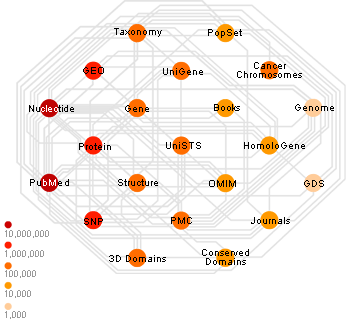
\includegraphics[width=1.0\textwidth]{drawings/entrez_datamodel.png}
        \end{center}
        \caption{Shows the structure of the Entrez datamodel}
        \label{EntrezDatamodel}
\end{figure}

\subsection{MedLine records and MeSH\label{MedLine_records_MeSH}}

\subsubsection{Overview}
MedLine (Medical Literature Analysis and Retrieval System Online)
\cite{PubMedFactSheetMedline} is the U.S. National Library of
Medicine's foremost bibliographic database, containing over 16 million
references to journal articles from approximately 5,200 journals
worldwide, dating from 1949 to the present. Since 2005 between
2,000-4,000 references have been added each Tuesday through Sunday and
over 670,000 references were added in 2007.

MedLine records are built from various fields such as title, abstract,
language, author, publication data and many others (for complete list
see \cite{PubMedHelpSearchFieldDescriptionsTags}). Using these search
fields, it is possible to specify exactly what is to be searched
for. As an example, the article could be one that needs to have an
abstract, has to have a specific author and is dated from 2005 and
later.

The records of MedLine are indexed with Medical Subject Headings
(MeSH) which is a controlled vocabulary thesaurus. MeSH describes a
hierarchical structure with the possibility of searching at different
levels of specificity. MeSH descriptors are very general at the
top-level (such as 'anatomy' or 'mental disorder') and gradually
becomes more and more specific when moving down its 11 levels (for
more information see their fact sheet on MeSH \cite{FactSheetMeSH}).
\fxnote{Der savnes et stoerre eksempel omkring MeSH records}

\subsubsection{Database interface}
When MeSH is used by experienced users, it can be a powerful tool to
extract information on a specific subject. But when used by less
experienced users, these tend to get long lists of hits which results
in an overload of information. For instance, a search on "Parkinson's
Disease" returns 21,000 results according to Panos et. al
\cite{DataMiningBiomedicine}. Panos et. al proposes a system that
divides MeSH into three categories, allowing multiple viewpoint \fxnote{daarlig formulering allowing multiple viewpoints} to
information \cite{DataMiningBiomedicine}. They cluster the results by
using a Self-Organizing Map thereby creating a concept hierarchy to
improve information retrieval.

There exists many different opinions when it comes to dealing with
MeSH in the context of information retrieval. W.R. Hersh and
D.H. Hickham found that text word indexing is more effective than MeSH
term indexing \cite{RetrievalEffectiveness}, while G. Sophie et. al
suggest that both MeSH and text search should be considered in the
search strategy \cite{FDGPET}.

Roger P. Smith describes how MeSH can be used to explode searches and
manipulate them to include the more specific sub levels of the
MeSH \cite{TheInternetforPhysicians}. For instance, a search for 'Filovirus' will include the more
specific searches 'Ebola virus' and 'Marburg virus'. The system tries
to correct user input errors through a system of mappings
(e.g. ``adverse reaction'', ``side effects'' and ``un-desirable
effects'' all map to ``adverse effects''). It is also possible to use
simple patterns when searching on PubMed, for example 'bacter*'
searches for bacteria, bacterium, bacteriophage etc. When using
truncation, the search will not find search strings containing
white-space, for example a search for 'infection*' will find
'infections', but not 'infection control'.

Though MedLine records are rich in information, we will in the system
be focusing on information given by the abstract, title and MeSH
terms. We require the records to have an abstract but MeSH terms might
not always be present. For an expansion of the prototype system, it
would be natural to take in account the information given with
potential keywords, publication dates, authors and other optional
MedLine information. \fxnote{Henvisning til ordentlig-syg
  implementerings afsnit i kap 3}

% <Figure/Table x.xx shows a typical Medline record>
\fxnote{InsertEither ref for appendix or a example of a medline record}

\subsection{Searching the information}
Having gathered information about rare diseases, our system needs to
be able to efficiently search and retrieve information given a query
string. Various approaches to retrieve the information needed
exists. A possibility is using boolean queries, where it is possible
to use the standard operators like ``AND'', ``OR'' and ``NOT'' to
perform queries a system --- this is the PubMed works. Many
professional users prefer using boolean queries, because it offers
them precise control over what is returned. Either a document matches
or it does not. But this does not mean that using boolean queries are
the most efficient, not even for professional searchers
\ref{IntroIR2009}. A problem is that the use of the ``AND'' operator
tends to produce high precision, but in turn lowers the recall of
information \ref{IntroIR2009}. As the boolean query model only record
term presence or absence, it lacks the ability to produce ranked
ordered results. In order to rank the query results the different
terms needs to be given a weight describing how important the term is
to the document. In order to incorporate the use of term weights, we
need to be able to calculate a relevans score for a document given a
query. A very popular way of doing this, is to represent the query and
documents in the collection as vectors. This leads us to choosing the
vector space model to represent our gathered information.

\section{The vector space model\label{VectorSpace}}

This model represents the way we structure all the retrieved
information that we use. It forms the backbone for the heuristics we
apply in the following chapters to model our data for an improved
search. We will in this section shortly describe its model (as used in
the prototype system), advantages and disadvantages.

\subsubsection{Model description}
The vector space model is a matrix representation of our
information. As shown in the figure below, each row represents a
document and each column a term.

% <Figure showing a term-doc matrix with no specific content>
\fxnote{Insert figure showing a term-doc matrix with no specific content}

In our case, the abstract, MeSH terms and title of a MedLine record
will represent a document vector in the model. The first index is
saved for a hash of the document id (PMID) \fxnote{Hash of the
  document id} while the remaining indices make up the term (or word)
frequencies of each term in the abstract, MeSH and title in the
record. The choice of putting the title of the record together with
its abstract is appropiate since these (often long) titles has a
tendency of carrying a lot of information on the MedLine records. As
described in section \ref{MedLine_records_MeSH}, the optional MeSH
also contains valuable information on the record.

Note also that the first index of each of the term vectors is saved
for the hash of the term.

\subsubsection{Advantages}
Representing our data in this model simplifies further
processing. It is a well known and well documented model (especially
due to its assumption of term independence which enables the use of naive
Bayes for document classification). It has several well researched and
used heuristics attached to it (like TF-IDF, section \ref{TFIDF} and LSA
 in section \ref{LSA}), and it is relatively easy to implement.

\subsubsection{Disadvantages}
As a basic model, the term vector scheme has several
limitations. First, it is very calculation intensive. We will try to
improve performance by using precalculated hashes of vector norms, by
stemming the terms and by removing outliers, but it still requires a
lot of processing time. Furthermore --- when we use schemes like
calculating the inverse document frequency --- updating the term space
leads to a recalculation of the entire matrix.

The matrix will also be very sparse, containing a lot more zeroes than
term frequencies. We will try to improve computational time and memory
by using data structures build for sparse matrices (see section
\ref{SciPy_sparse}). 

Another main disadvantage of the vector space model is that it does
not capture polysemy\footnote{Polysemy describes terms that can be
  used to express different things in different contexts,
  e.g. \textit{driving a car} and \textit{driving results}. } or
synonymity, since every term is assumed independent. Thus some
irrelevant documents have high similarities with a query because they
share some words with the query (polysemy) while other relevant
documents have a low similarity with the query since they have
different terms (synonymy).  Lack of polysemy comprehension affects
the recall of a search on the model. Lack of synonymy comprehension
affects the precision of a search. Some synonyms can be caught by
stemming the terms but far from all. We will also to create a
semantic space using SVD (see section \ref{LSA}) to capture the most
meaningful words.

\section{Applied heuristics}

There exists many heuristics for information processing that can be
used when dealing with term-document matrices and the vector space
model. In this section, we will go through some of the most commonly
used schemes for enhancing the performance (recall and precision) of a
search in the model. We will also go through some less common schemes
used for the prototype system and justify these decisions.

\subsection{Mitigating the problem of term burstiness\label{MitigatingBurstiness}}

The term 'burstiness' describes the behavior of a rare word appearing
many times in a single document according to Rasmus E. Madsen et. al
\cite{ModelingWordBurstiness2005}. This is under the general
assumption that if a word appears once in a document, it is more
likely to appear again. This assumption breaks with the independence
assumption of the vector space model and a high raw count of a word
often seems to exaggerate the significance of that word. Derived from
\cite{ModelingWordBurstiness2005}, our first heuristic is the
log-transformation of the term frequency:

\[
x_{dw}^{log} = \log{(1 + x_{dw})}
\]

Where $x_{dw}$ is the number of times the term $w$ appears in document
$d$. This helps reduce the problem of burstiness by smoothing \fxnote{find other word than smoothing} the term
counts.

\subsection{Term Frequency - Inverse Document Frequency\label{TFIDF}}

This heuristic is commonly known under the acronym TF-IDF and is
probably the most used heuristic in the vector space model and
information retrieval in general. It looks as follows (note also the
log-transformation of the term frequency from
section \ref{MitigatingBurstiness}):

\[
x_{ij}^{tfidf} = \log{(1 + x_{dw})} * \log{\frac{D}{\sum_{d\prime = 1}^{D}\delta_{d\prime w}} }
\]

Where $\delta_{dw}$ is $1$ if $w$ is present in document $d$ and $D$
is the document corpus. Term frequency ($\mathit{tf}$) is also referred to as the
\textit{recall} component while the inverse document frequency (IDF)
is the \textit{precision} component. In other words, IDF gives us a
higher weight for rare terms and the log-transformation of IDF helps
to smooth \fxnote{Find andet ord end to smooth} the data. With TF-IDF the importance increases
proportionally to the number of times a term appears in the document
but is offset by the frequency of the word in the corpus.

One clear disadvantage of TF-IDF is its inability to capture the
importance of a term. Though rare words a promoted, there is no real
guarantee that these words are as relevant and classifying for the
document as one could hope. A lot of research have been laid into
explaining the advantages and disadvantages of TF-IDF and there are
many interesting discussions going on --- like the one at the blog
\cite{UnderstandingTFIDF} --- in this discussion, it would make sense
to work with some measure of the entropy of a term but --- as also
noted --- such methods are computationally expensive, especially when
dealing with large scale web search engines. It would be reasonable to
assume that the same applies when dealing with large term document
matrices and --- due to the limited resources available in this
project --- we believe it is reason enough to only consider the
relatively simple transformations.

\subsection{Normalization} 

After the TF-IDF transformation, there is a need to normalize the
vectors using L$_2$ normalization\footnote{Also known as the
  Euclidian norm}. This makes all the document vectors have the same
length and therefore the same influence on the search result.

\[
x_{dw}^{norm} = \frac{x_{dw}^{tfidf}}{\sqrt{\sum_{w\prime = 1}^{W} {x_{dw}^{tfidf}}^{2}}}
\]

Where $\sqrt{\sum_{w\prime = 1}^{W} {x_{dw}^{tfidf}}^{2}}$ is the
normalization factor of the $x_{dw}^{tfidf}$ - using the usual vector
normalization to make the length 1.

\subsection{Square root transformation\label{SquareRoot}}

Like the log-transformation in section \ref{MitigatingBurstiness}, the square
root transformation represents a method for smoothing burstiness in
data. The most important difference is that using the square root on
data smoothes the data towards 1 as a contrast to the more aggresive
log-transformation. Numbers of 1 and above behave differently than
numbers between 0.00 and 0.99. The square root of numbers above 1.00
always become smaller, 1 and 0 remain constant, and numbers
between 0.00 and 1.00 become larger (the square root of 4 is 2, but
the square root of 0.40 is 0.63). Thus the square root transformation
should only be used on data that is either below or above 1.

\fxnote{make a figure of sqrt(x) and insert here.}

We will be using the square root transformation to analyse the data
coming from the TF-IDF scheme. We will describe transformation in
further detail in chapter \ref{ExperimentsResults} \fxnote{Might want
  to ref to section}. For now, the basic idea is that --- if the TF-IDF
works as supposed --- a square root 'upping' of the lower data will
result in poorer search results.

\subsection{Stop word removal}

We will be removing english stop words in the prototype to limit the
number of too common words that interfere with searches. In recent
years there has been a tendency to avoid using stop word removal due
to the small impact that it has on a search \cite{IntroIR2009}. But
taking into consideration that most searches performed on this system
will consist of a list of symptoms, it seems that it will not damage
the performance of the system to remove the insignificant terms
(remember the assumption of term independence). In any case, these
terms --- like 'and' or 'this' --- would be present in nearly all of
the MedLine records and therefore be assigned very low weight by
TF-IDF. Let us for instance say that the term 'a' was present in every
document. The IDF-factor would be $\log 1 = 0$ which results in
$\mathit{tf} \times \mathit{idf} = \mathit{tf} \times 0 = 0$. The term
will therefore be deemed irrelevant in relation to the information
retrieval.

\subsection{Stemming}

Performing stemming on textual information will increase the recall of
information at the price of lowering the
precision\footnote{Remembering from section \ref{TFIDF} could be
  defined as TF and precision as IDF in the TF-IDF vector space model}
\cite{IntroIR2009}. Considering that our system will be dealing with
domain specific information, it should not pose a problem. Our choice
of stemmer has fallen on Porter's stemmer which has also been shown
empirically to be very efficient \cite{IntroIR2009}. Other stemmers
exists --- like Lovins which is the first stemmer to be made and is
very aggressive in its stemming \cite{Kurz2002309}. Or like the simple
S stemmer --- for English words --- where only endings of common words
are stemmed such as 'ies', 'es' and 's'. A complete alternative using
a stemmer could be to use a lemmatizer. A lemmatizer performs a full
morphological analysis to accurately identify the lemma of a word. Performing
lemmatization seems to have only very limited benefits for the
retrieval \cite{IntroIR2009}. For our system, we have chosen to stick with only
testing stemming.

\subsection{Outlier detection}

Outlier detection on the retrieved information of each disease could
concentrate the knowledge that we have on the disease. But care needs
to be taken when removing information since there is the risk of
removing specific terms required to identify the correct
disease. There are multiple ways of performing outlier detection, the
most interesting generally being the most computationally
expensive. One way could be to make a centroid vector for each disease
and then remove a percentage of the MedLine records farthest away from
the centroid by choosing some similarity/distance measure on which to
score them. Cosine Similarity (see section \ref{VectorSimilarity})
would be well suited for the purpose. Another way could be to
calculate a distance matrix from each document vector to all others,
again using an appropriate distance measure like the cosine similarity
(see section \ref{VectorSimilarity}). This is then followed by taking
the sum of each document vector and removing the percentage that score
the lowest, that is the ones that --- summed over all distances to
every other document vector --- scores the lowest. 

\fxnote{Do we do outlier detection, not yet!}  We will be
experimenting with outlier detection but it is not a primary focus,
since --- without a classifier --- it is impossible to guarantee the
removed documents are irrelevant.

\subsection{Latent Semantic Analysis\label{LSA}}

Additional interesting preprocessing would be to create a latent
semantic space on the information on each disease. This can be done by
performing latent semantic analysis (LSA)/latent semantic indexing
(LSI). With this scheme, it should be possible to extract a keyword
list describing each disease or summarizing the information we have
available about the disease. The keyword list could then be used to
provide the physician using the system with a more comprehensive list
of characteristics for the most likely diseases, given the original
symptoms. It could be used for later disease classification schemes.

LSA is done by performing Singular Value Decomposition (SVD). SVD
decomposes the original matrix X, with shape $\mathit{m}$ x
$\mathit{n}$, into a product of three new matrices $U$, $S$ and
$V^{t}$. Here $U$ is an $\mathit{m}$ x $\mathit{n}$ matrix, $S$ is an
$\mathit{n}$ x $\mathit{n}$ diagonal matrix and $V^{t}$ is an
$\mathit{n}$ x $\mathit{n}$ matrix. The column of $U$ is called left
singular vectors, and the rows of $V^{t}$ is called right singular
vectors. The elements of $S$ are only nonzero on the diagonal and
these are called singular values. The singular values are the square
root of the eigenvalues of $X^{t}X$, arranged in decreasing order. A
dimension reduction is performed by removing the $k$ least significant
singular values, the $k$ last columns of $U$, and the $k$ last rows of
$V^{t}$. The result is an $n - k = l$ matrix where $l$ is the
remaining dimensions. Due to the reduction, the dimensions are now
$U_{r}$ is $\mathit{m}$ x $\mathit{l}$, $S_{r}$ is $\mathit{l}$ x
$\mathit{l}$, and $V_{r}^{t}$ is $\mathit{l}$ x $\mathit{n}$. SVD ---
and the dimensionality reduction --- is then followed by calculating
the product of $U_{r}S_{r}V_{r}^{t}$ (where the subscribtion $_{r}$
means reduced), hence putting the three reformed pieces back together:

\[
X_{r} = U_{r}S_{r}V_{r}^{t}, \textrm{ where } X \textrm{ is } m \textrm{ x }n
\]

$X_{r}$ is also called the semantic space, and should --- in theory --- be
able capture some of the semantic relation between terms.

\section{Calculation of vector similarity\label{VectorSimilarity}}

When working with the vector space model, the most used measure of
similarity is the cosine similarity. In the prototype system, we use
this measure for scoring and clustering diseases based on queries. We
also use a simpler \textit{sum} score in comparison with the cosine
measure.

\subsubsection{The cosine similarity measure}
When using this measure, the resulting similarity score of two vectors
can be thought of as the angle between two vectors (though the angle
measure is only visible for up to three dimensions and can not readily
be applied to the hyper dimensional space of the matrix), i.e. the
angle between the query vector and the document vector. The usual
equation for cosine similarity can then be used:

\[
\cos \theta_{D_j} = \frac{Q \cdot D_j}{|Q| \times |D_j|}
\]

Where $D_j$ is document $j$ as a vector, $Q$ is the query vector and
$\cos \theta_{D_{j}}$ is the cosine similarity between document $j$ and
query $Q$.

Since we assume that no values in the vector space model are
below zero, this measure results in a value of 0 if the vectors have
no terms in common and 1 if they are exactly like each other. The
latter case is most improbable in our proposed system since the query
vector usually consists of a limited list of symptoms, measured up
against the document vector consisting of a long list of terms derived
from the title, the abstract and the potential MeSH terms of a MedLine
record.

With a TF-IDF transformation and L$_2$ normalization the above
calculation can be rewritten as follows: 

\[
\textrm{score}_{d} = \frac{1}{|I|}\frac{1}{|x_{d}|} \sum_{i \in I} x_{dw}
\]

Where $\textrm{score}_{d}$ is the similarity score for document $d$,
$\frac{1}{|I|}$ is the normalization factor of the query vector and
$\frac{1}{|x_{d}|}$ is the normalization factor of the document
vector. Due to the fact that length of the query vector is the same
for all the document vectors in a given search, this acts as a scalar
for all scores. Because of this we choose to disregard the
$\frac{1}{|I|}$ factor in our system, meaning we can rewrite the
formula to:

\[
\propto \frac{\sum_{i \in I} x_{dw}} {|x_{d}|}
\]

Since the denominator is the norm of the document vector, the division
above simply represents a normalization of the document vector so that
it is on unit length. To improve query processing time, the
normalization of the document corpus matrix --- that we will be working
on --- can be preprocessed before the calculation of the cosine
similarity. Assuming that the document vectors are on unit length, we
can now rewrite the cosine similarity function to be on the simple
form: 

\[
\propto  \sum_{i \in I} \widehat{x_{dw}}
\]

Where $I$ is the set of indices where query vector and document vector
overlap. And $\widehat{x_{dw}}$ is the normalized version of $x_{dw}$

If there should arise the need to compare two searches, there is of
course a need to normalize the search score in accordance to the
length of the query vector.

How we use the cosine similarity measure to test and score our data
will be described in chapter \ref{ExperimentsResults}.

\fxnote{REF: om scoring i experimental chap}

\subsubsection{The simple sum measure\label{SimpleSum}}
When using this measure, we simply sum the vectors values returned by
a query. In other words, this works like the cosine measure described
above but it deals with non-normalized vector spaces as a contrary to
the cosine measure. This will also be described in chapter
\fxnote{REF: om scoring i experimental chap.}.

\section{Data structures}

When constructing a term document matrix, it is essential to use the
right data structures to save the information. Creating a term
document matrix from diverse MedLine records tends to produce very
large sparse matrix. One of the matrices (a stemmed version) that we
will be creating has shown to contain only about 0.026\% non-zero
entries, corresponding to about 61,520,349 term counts in a matrix for
size 602,467(documents)x390.766(terms) with a total capacity of
235,423,619,722 entries. In short, this means a lot of zeroes. Working
with a matrix that takes all these zeroes into account is simply not
an option. For saving time and space we have chosen to work with three
main data structures.

\subsection{SciPy.sparse\label{SciPy_sparse}}

The SciPy.sparse module is used to make sparse matrices. It offers
seven different forms of data structures to represent sparse matrices
- the interested reader can have a look at the SciPy documentation
accessible at their website \cite{SciPy}. The different types each have pros and
cons. We primarily use the "lil" format, which is a sparse matrix
using linked lists. For traversal through the matrix, we use the "coo"
format which is coordinate format. coo matrices also facilitate fast
conversion to the other matrix format. For a quick look-up of
individual elements, it is advantagous to use the "dok" format which
is a dictionary of keys. This allows O(1) time access to matrix
elements. And the "csc" and "csr" formats can be used when dealing
with arithmetic operations since these are efficient for column and
row operations.

Linked list matrices are slow when it comes to arithmetic
operations but efficient when it comes to incrementally constructing
matrices. Therefore it is ideal to construct a large matrix from a
number of smaller matrices using linked list format. It also permits
the usage of fancy slicing which makes manipulations of the content
very flexible. When the construction is done, it can be converted to
another format for efficient arithmetic operations (usually csc or
csr). The lil format also tends to have a high memory usage than the
other sparse matrix formats.

Coordinate matrices are memory efficient but does not allow for
direct access to the elements it contains. It is however possible to
traverse over all the elements which is useful when constructing a
term document matrix. This is especially fast when combined with the
dok format which allows fast access for elements.

Compressed sparse row or column allows for fast matrix
arithmetic operations like, addition, multiplication, matrix matrix
product, vector matrix product and so on. The csr allow fast row
slicing but is slow when column slicing and csc vice versa.

The two remaining sparse matrix formats in SciPy are not relevant to the
project.

\subsection{Matrix Market\label{MatrixMarket}}

Revisiting the discussion on how to save the term document matrix, the
Scipy package \cite{SciPy} offers an I/O-module that allows matrices
to be exported to "Matrix Market" (MM) format. MM that only saves
non-zero entries via coordinate/value. When reading in from an MM
file, the matrix is read in is in coo format for obvious
reasons\footnote{The exception being the "dense" format, which is
  similar NumPy's matrix format.}. More information can be found at
their website \cite{MatrixMarket}.

\subsection{cPickle}

cPickle is a standard Python module that is used for serializing
Python objects. It can be used to save objects to the harddrive and
later read them back into memory - without bothering with type
transformations. cPickle has the unfortunate property that it saves
all the zeroes that resides within the term document matrix which
results in large files. Fortunately cPickle is very efficient when it
comes to saving and reading the hashes that we use for the
matrices. The I/O time is pretty quick and it enables a much quicker
read of the hashes than, say a plain text file would have. More on
cPickle can be found at Python's documentation site
\cite{cPicklePython}.

\subsection{The Orpha.net alternative\label{Orphanet}}

Though we have chosen Rarediseases.info to harvest much of our data from, 
we have also come across another website worthy of mention as it seems 
this site is more rich in information than Rarediseases.info - though 
focused on rare diseases in Europe.

Orpha.net defines a rare disease as one that affects 1 person out of 
every 2,000 in Europe and it lists 12,191 different rare diseases at 
the time of writing. A quick overview suggests more of the detailed 
descriptions than Rarediseases.info and it has highlighted data such 
as "Prevalence of rare diseases" and "Age of onset" which could be very 
useful for disease classification. Like Rarediseases.info it is 
--- however --- variable in the amount of information per disease and 
not all diseases have any information on them, say for its name.

Since Orpha.net focuses on diseases that are rare in Europe, a combination 
of data from Raredisease.info and Orpha.net could enable a physician using 
the system to enhance the precision by defining the continental origin of 
the disease. It could also up the number of diseases with a description to 
a large enough amount for a classifier to use them for priors in a 
statistical model. 
